\documentclass[10pt]{article}
\usepackage{tmlr}
% \usepackage[accepted]{tmlr}
% \usepackage[preprint]{tmlr}

\usepackage[utf8]{inputenc}
\usepackage[T1]{fontenc}
%%%%% NEW MATH DEFINITIONS %%%%%

\usepackage{amsmath,amsfonts,bm}

% Mark sections of captions for referring to divisions of figures
\newcommand{\figleft}{{\em (Left)}}
\newcommand{\figcenter}{{\em (Center)}}
\newcommand{\figright}{{\em (Right)}}
\newcommand{\figtop}{{\em (Top)}}
\newcommand{\figbottom}{{\em (Bottom)}}
\newcommand{\captiona}{{\em (a)}}
\newcommand{\captionb}{{\em (b)}}
\newcommand{\captionc}{{\em (c)}}
\newcommand{\captiond}{{\em (d)}}

% Highlight a newly defined term
\newcommand{\newterm}[1]{{\bf #1}}


% Figure reference, lower-case.
\def\figref#1{figure~\ref{#1}}
% Figure reference, capital. For start of sentence
\def\Figref#1{Figure~\ref{#1}}
\def\twofigref#1#2{figures \ref{#1} and \ref{#2}}
\def\quadfigref#1#2#3#4{figures \ref{#1}, \ref{#2}, \ref{#3} and \ref{#4}}
% Section reference, lower-case.
\def\secref#1{section~\ref{#1}}
% Section reference, capital.
\def\Secref#1{Section~\ref{#1}}
% Reference to two sections.
\def\twosecrefs#1#2{sections \ref{#1} and \ref{#2}}
% Reference to three sections.
\def\secrefs#1#2#3{sections \ref{#1}, \ref{#2} and \ref{#3}}
% Reference to an equation, lower-case.
\def\eqref#1{equation~\ref{#1}}
% Reference to an equation, upper case
\def\Eqref#1{Equation~\ref{#1}}
% A raw reference to an equation---avoid using if possible
\def\plaineqref#1{\ref{#1}}
% Reference to a chapter, lower-case.
\def\chapref#1{chapter~\ref{#1}}
% Reference to an equation, upper case.
\def\Chapref#1{Chapter~\ref{#1}}
% Reference to a range of chapters
\def\rangechapref#1#2{chapters\ref{#1}--\ref{#2}}
% Reference to an algorithm, lower-case.
\def\algref#1{algorithm~\ref{#1}}
% Reference to an algorithm, upper case.
\def\Algref#1{Algorithm~\ref{#1}}
\def\twoalgref#1#2{algorithms \ref{#1} and \ref{#2}}
\def\Twoalgref#1#2{Algorithms \ref{#1} and \ref{#2}}
% Reference to a part, lower case
\def\partref#1{part~\ref{#1}}
% Reference to a part, upper case
\def\Partref#1{Part~\ref{#1}}
\def\twopartref#1#2{parts \ref{#1} and \ref{#2}}

\def\ceil#1{\lceil #1 \rceil}
\def\floor#1{\lfloor #1 \rfloor}
\def\1{\bm{1}}
\newcommand{\train}{\mathcal{D}}
\newcommand{\valid}{\mathcal{D_{\mathrm{valid}}}}
\newcommand{\test}{\mathcal{D_{\mathrm{test}}}}

\def\eps{{\epsilon}}


% Random variables
\def\reta{{\textnormal{$\eta$}}}
\def\ra{{\textnormal{a}}}
\def\rb{{\textnormal{b}}}
\def\rc{{\textnormal{c}}}
\def\rd{{\textnormal{d}}}
\def\re{{\textnormal{e}}}
\def\rf{{\textnormal{f}}}
\def\rg{{\textnormal{g}}}
\def\rh{{\textnormal{h}}}
\def\ri{{\textnormal{i}}}
\def\rj{{\textnormal{j}}}
\def\rk{{\textnormal{k}}}
\def\rl{{\textnormal{l}}}
% rm is already a command, just don't name any random variables m
\def\rn{{\textnormal{n}}}
\def\ro{{\textnormal{o}}}
\def\rp{{\textnormal{p}}}
\def\rq{{\textnormal{q}}}
\def\rr{{\textnormal{r}}}
\def\rs{{\textnormal{s}}}
\def\rt{{\textnormal{t}}}
\def\ru{{\textnormal{u}}}
\def\rv{{\textnormal{v}}}
\def\rw{{\textnormal{w}}}
\def\rx{{\textnormal{x}}}
\def\ry{{\textnormal{y}}}
\def\rz{{\textnormal{z}}}

% Random vectors
\def\rvepsilon{{\mathbf{\epsilon}}}
\def\rvtheta{{\mathbf{\theta}}}
\def\rva{{\mathbf{a}}}
\def\rvb{{\mathbf{b}}}
\def\rvc{{\mathbf{c}}}
\def\rvd{{\mathbf{d}}}
\def\rve{{\mathbf{e}}}
\def\rvf{{\mathbf{f}}}
\def\rvg{{\mathbf{g}}}
\def\rvh{{\mathbf{h}}}
\def\rvu{{\mathbf{i}}}
\def\rvj{{\mathbf{j}}}
\def\rvk{{\mathbf{k}}}
\def\rvl{{\mathbf{l}}}
\def\rvm{{\mathbf{m}}}
\def\rvn{{\mathbf{n}}}
\def\rvo{{\mathbf{o}}}
\def\rvp{{\mathbf{p}}}
\def\rvq{{\mathbf{q}}}
\def\rvr{{\mathbf{r}}}
\def\rvs{{\mathbf{s}}}
\def\rvt{{\mathbf{t}}}
\def\rvu{{\mathbf{u}}}
\def\rvv{{\mathbf{v}}}
\def\rvw{{\mathbf{w}}}
\def\rvx{{\mathbf{x}}}
\def\rvy{{\mathbf{y}}}
\def\rvz{{\mathbf{z}}}

% Elements of random vectors
\def\erva{{\textnormal{a}}}
\def\ervb{{\textnormal{b}}}
\def\ervc{{\textnormal{c}}}
\def\ervd{{\textnormal{d}}}
\def\erve{{\textnormal{e}}}
\def\ervf{{\textnormal{f}}}
\def\ervg{{\textnormal{g}}}
\def\ervh{{\textnormal{h}}}
\def\ervi{{\textnormal{i}}}
\def\ervj{{\textnormal{j}}}
\def\ervk{{\textnormal{k}}}
\def\ervl{{\textnormal{l}}}
\def\ervm{{\textnormal{m}}}
\def\ervn{{\textnormal{n}}}
\def\ervo{{\textnormal{o}}}
\def\ervp{{\textnormal{p}}}
\def\ervq{{\textnormal{q}}}
\def\ervr{{\textnormal{r}}}
\def\ervs{{\textnormal{s}}}
\def\ervt{{\textnormal{t}}}
\def\ervu{{\textnormal{u}}}
\def\ervv{{\textnormal{v}}}
\def\ervw{{\textnormal{w}}}
\def\ervx{{\textnormal{x}}}
\def\ervy{{\textnormal{y}}}
\def\ervz{{\textnormal{z}}}

% Random matrices
\def\rmA{{\mathbf{A}}}
\def\rmB{{\mathbf{B}}}
\def\rmC{{\mathbf{C}}}
\def\rmD{{\mathbf{D}}}
\def\rmE{{\mathbf{E}}}
\def\rmF{{\mathbf{F}}}
\def\rmG{{\mathbf{G}}}
\def\rmH{{\mathbf{H}}}
\def\rmI{{\mathbf{I}}}
\def\rmJ{{\mathbf{J}}}
\def\rmK{{\mathbf{K}}}
\def\rmL{{\mathbf{L}}}
\def\rmM{{\mathbf{M}}}
\def\rmN{{\mathbf{N}}}
\def\rmO{{\mathbf{O}}}
\def\rmP{{\mathbf{P}}}
\def\rmQ{{\mathbf{Q}}}
\def\rmR{{\mathbf{R}}}
\def\rmS{{\mathbf{S}}}
\def\rmT{{\mathbf{T}}}
\def\rmU{{\mathbf{U}}}
\def\rmV{{\mathbf{V}}}
\def\rmW{{\mathbf{W}}}
\def\rmX{{\mathbf{X}}}
\def\rmY{{\mathbf{Y}}}
\def\rmZ{{\mathbf{Z}}}

% Elements of random matrices
\def\ermA{{\textnormal{A}}}
\def\ermB{{\textnormal{B}}}
\def\ermC{{\textnormal{C}}}
\def\ermD{{\textnormal{D}}}
\def\ermE{{\textnormal{E}}}
\def\ermF{{\textnormal{F}}}
\def\ermG{{\textnormal{G}}}
\def\ermH{{\textnormal{H}}}
\def\ermI{{\textnormal{I}}}
\def\ermJ{{\textnormal{J}}}
\def\ermK{{\textnormal{K}}}
\def\ermL{{\textnormal{L}}}
\def\ermM{{\textnormal{M}}}
\def\ermN{{\textnormal{N}}}
\def\ermO{{\textnormal{O}}}
\def\ermP{{\textnormal{P}}}
\def\ermQ{{\textnormal{Q}}}
\def\ermR{{\textnormal{R}}}
\def\ermS{{\textnormal{S}}}
\def\ermT{{\textnormal{T}}}
\def\ermU{{\textnormal{U}}}
\def\ermV{{\textnormal{V}}}
\def\ermW{{\textnormal{W}}}
\def\ermX{{\textnormal{X}}}
\def\ermY{{\textnormal{Y}}}
\def\ermZ{{\textnormal{Z}}}

% Vectors
\def\vzero{{\bm{0}}}
\def\vone{{\bm{1}}}
\def\vmu{{\bm{\mu}}}
\def\vtheta{{\bm{\theta}}}
\def\va{{\bm{a}}}
\def\vb{{\bm{b}}}
\def\vc{{\bm{c}}}
\def\vd{{\bm{d}}}
\def\ve{{\bm{e}}}
\def\vf{{\bm{f}}}
\def\vg{{\bm{g}}}
\def\vh{{\bm{h}}}
\def\vi{{\bm{i}}}
\def\vj{{\bm{j}}}
\def\vk{{\bm{k}}}
\def\vl{{\bm{l}}}
\def\vm{{\bm{m}}}
\def\vn{{\bm{n}}}
\def\vo{{\bm{o}}}
\def\vp{{\bm{p}}}
\def\vq{{\bm{q}}}
\def\vr{{\bm{r}}}
\def\vs{{\bm{s}}}
\def\vt{{\bm{t}}}
\def\vu{{\bm{u}}}
\def\vv{{\bm{v}}}
\def\vw{{\bm{w}}}
\def\vx{{\bm{x}}}
\def\vy{{\bm{y}}}
\def\vz{{\bm{z}}}

% Elements of vectors
\def\evalpha{{\alpha}}
\def\evbeta{{\beta}}
\def\evepsilon{{\epsilon}}
\def\evlambda{{\lambda}}
\def\evomega{{\omega}}
\def\evmu{{\mu}}
\def\evpsi{{\psi}}
\def\evsigma{{\sigma}}
\def\evtheta{{\theta}}
\def\eva{{a}}
\def\evb{{b}}
\def\evc{{c}}
\def\evd{{d}}
\def\eve{{e}}
\def\evf{{f}}
\def\evg{{g}}
\def\evh{{h}}
\def\evi{{i}}
\def\evj{{j}}
\def\evk{{k}}
\def\evl{{l}}
\def\evm{{m}}
\def\evn{{n}}
\def\evo{{o}}
\def\evp{{p}}
\def\evq{{q}}
\def\evr{{r}}
\def\evs{{s}}
\def\evt{{t}}
\def\evu{{u}}
\def\evv{{v}}
\def\evw{{w}}
\def\evx{{x}}
\def\evy{{y}}
\def\evz{{z}}

% Matrix
\def\mA{{\bm{A}}}
\def\mB{{\bm{B}}}
\def\mC{{\bm{C}}}
\def\mD{{\bm{D}}}
\def\mE{{\bm{E}}}
\def\mF{{\bm{F}}}
\def\mG{{\bm{G}}}
\def\mH{{\bm{H}}}
\def\mI{{\bm{I}}}
\def\mJ{{\bm{J}}}
\def\mK{{\bm{K}}}
\def\mL{{\bm{L}}}
\def\mM{{\bm{M}}}
\def\mN{{\bm{N}}}
\def\mO{{\bm{O}}}
\def\mP{{\bm{P}}}
\def\mQ{{\bm{Q}}}
\def\mR{{\bm{R}}}
\def\mS{{\bm{S}}}
\def\mT{{\bm{T}}}
\def\mU{{\bm{U}}}
\def\mV{{\bm{V}}}
\def\mW{{\bm{W}}}
\def\mX{{\bm{X}}}
\def\mY{{\bm{Y}}}
\def\mZ{{\bm{Z}}}
\def\mBeta{{\bm{\beta}}}
\def\mPhi{{\bm{\Phi}}}
\def\mLambda{{\bm{\Lambda}}}
\def\mSigma{{\bm{\Sigma}}}

% Tensor
\DeclareMathAlphabet{\mathsfit}{\encodingdefault}{\sfdefault}{m}{sl}
\SetMathAlphabet{\mathsfit}{bold}{\encodingdefault}{\sfdefault}{bx}{n}
\newcommand{\tens}[1]{\bm{\mathsfit{#1}}}
\def\tA{{\tens{A}}}
\def\tB{{\tens{B}}}
\def\tC{{\tens{C}}}
\def\tD{{\tens{D}}}
\def\tE{{\tens{E}}}
\def\tF{{\tens{F}}}
\def\tG{{\tens{G}}}
\def\tH{{\tens{H}}}
\def\tI{{\tens{I}}}
\def\tJ{{\tens{J}}}
\def\tK{{\tens{K}}}
\def\tL{{\tens{L}}}
\def\tM{{\tens{M}}}
\def\tN{{\tens{N}}}
\def\tO{{\tens{O}}}
\def\tP{{\tens{P}}}
\def\tQ{{\tens{Q}}}
\def\tR{{\tens{R}}}
\def\tS{{\tens{S}}}
\def\tT{{\tens{T}}}
\def\tU{{\tens{U}}}
\def\tV{{\tens{V}}}
\def\tW{{\tens{W}}}
\def\tX{{\tens{X}}}
\def\tY{{\tens{Y}}}
\def\tZ{{\tens{Z}}}


% Graph
\def\gA{{\mathcal{A}}}
\def\gB{{\mathcal{B}}}
\def\gC{{\mathcal{C}}}
\def\gD{{\mathcal{D}}}
\def\gE{{\mathcal{E}}}
\def\gF{{\mathcal{F}}}
\def\gG{{\mathcal{G}}}
\def\gH{{\mathcal{H}}}
\def\gI{{\mathcal{I}}}
\def\gJ{{\mathcal{J}}}
\def\gK{{\mathcal{K}}}
\def\gL{{\mathcal{L}}}
\def\gM{{\mathcal{M}}}
\def\gN{{\mathcal{N}}}
\def\gO{{\mathcal{O}}}
\def\gP{{\mathcal{P}}}
\def\gQ{{\mathcal{Q}}}
\def\gR{{\mathcal{R}}}
\def\gS{{\mathcal{S}}}
\def\gT{{\mathcal{T}}}
\def\gU{{\mathcal{U}}}
\def\gV{{\mathcal{V}}}
\def\gW{{\mathcal{W}}}
\def\gX{{\mathcal{X}}}
\def\gY{{\mathcal{Y}}}
\def\gZ{{\mathcal{Z}}}

% Sets
\def\sA{{\mathbb{A}}}
\def\sB{{\mathbb{B}}}
\def\sC{{\mathbb{C}}}
\def\sD{{\mathbb{D}}}
% Don't use a set called E, because this would be the same as our symbol
% for expectation.
\def\sF{{\mathbb{F}}}
\def\sG{{\mathbb{G}}}
\def\sH{{\mathbb{H}}}
\def\sI{{\mathbb{I}}}
\def\sJ{{\mathbb{J}}}
\def\sK{{\mathbb{K}}}
\def\sL{{\mathbb{L}}}
\def\sM{{\mathbb{M}}}
\def\sN{{\mathbb{N}}}
\def\sO{{\mathbb{O}}}
\def\sP{{\mathbb{P}}}
\def\sQ{{\mathbb{Q}}}
\def\sR{{\mathbb{R}}}
\def\sS{{\mathbb{S}}}
\def\sT{{\mathbb{T}}}
\def\sU{{\mathbb{U}}}
\def\sV{{\mathbb{V}}}
\def\sW{{\mathbb{W}}}
\def\sX{{\mathbb{X}}}
\def\sY{{\mathbb{Y}}}
\def\sZ{{\mathbb{Z}}}

% Entries of a matrix
\def\emLambda{{\Lambda}}
\def\emA{{A}}
\def\emB{{B}}
\def\emC{{C}}
\def\emD{{D}}
\def\emE{{E}}
\def\emF{{F}}
\def\emG{{G}}
\def\emH{{H}}
\def\emI{{I}}
\def\emJ{{J}}
\def\emK{{K}}
\def\emL{{L}}
\def\emM{{M}}
\def\emN{{N}}
\def\emO{{O}}
\def\emP{{P}}
\def\emQ{{Q}}
\def\emR{{R}}
\def\emS{{S}}
\def\emT{{T}}
\def\emU{{U}}
\def\emV{{V}}
\def\emW{{W}}
\def\emX{{X}}
\def\emY{{Y}}
\def\emZ{{Z}}
\def\emSigma{{\Sigma}}

% entries of a tensor
% Same font as tensor, without \bm wrapper
\newcommand{\etens}[1]{\mathsfit{#1}}
\def\etLambda{{\etens{\Lambda}}}
\def\etA{{\etens{A}}}
\def\etB{{\etens{B}}}
\def\etC{{\etens{C}}}
\def\etD{{\etens{D}}}
\def\etE{{\etens{E}}}
\def\etF{{\etens{F}}}
\def\etG{{\etens{G}}}
\def\etH{{\etens{H}}}
\def\etI{{\etens{I}}}
\def\etJ{{\etens{J}}}
\def\etK{{\etens{K}}}
\def\etL{{\etens{L}}}
\def\etM{{\etens{M}}}
\def\etN{{\etens{N}}}
\def\etO{{\etens{O}}}
\def\etP{{\etens{P}}}
\def\etQ{{\etens{Q}}}
\def\etR{{\etens{R}}}
\def\etS{{\etens{S}}}
\def\etT{{\etens{T}}}
\def\etU{{\etens{U}}}
\def\etV{{\etens{V}}}
\def\etW{{\etens{W}}}
\def\etX{{\etens{X}}}
\def\etY{{\etens{Y}}}
\def\etZ{{\etens{Z}}}

% The true underlying data generating distribution
\newcommand{\pdata}{p_{\rm{data}}}
% The empirical distribution defined by the training set
\newcommand{\ptrain}{\hat{p}_{\rm{data}}}
\newcommand{\Ptrain}{\hat{P}_{\rm{data}}}
% The model distribution
\newcommand{\pmodel}{p_{\rm{model}}}
\newcommand{\Pmodel}{P_{\rm{model}}}
\newcommand{\ptildemodel}{\tilde{p}_{\rm{model}}}
% Stochastic autoencoder distributions
\newcommand{\pencode}{p_{\rm{encoder}}}
\newcommand{\pdecode}{p_{\rm{decoder}}}
\newcommand{\precons}{p_{\rm{reconstruct}}}

\newcommand{\laplace}{\mathrm{Laplace}} % Laplace distribution

\newcommand{\E}{\mathbb{E}}
\newcommand{\Ls}{\mathcal{L}}
\newcommand{\R}{\mathbb{R}}
\newcommand{\emp}{\tilde{p}}
\newcommand{\lr}{\alpha}
\newcommand{\reg}{\lambda}
\newcommand{\rect}{\mathrm{rectifier}}
\newcommand{\softmax}{\mathrm{softmax}}
\newcommand{\sigmoid}{\sigma}
\newcommand{\softplus}{\zeta}
\newcommand{\KL}{D_{\mathrm{KL}}}
\newcommand{\Var}{\mathrm{Var}}
\newcommand{\standarderror}{\mathrm{SE}}
\newcommand{\Cov}{\mathrm{Cov}}
% Wolfram Mathworld says $L^2$ is for function spaces and $\ell^2$ is for vectors
% But then they seem to use $L^2$ for vectors throughout the site, and so does
% wikipedia.
\newcommand{\normlzero}{L^0}
\newcommand{\normlone}{L^1}
\newcommand{\normltwo}{L^2}
\newcommand{\normlp}{L^p}
\newcommand{\normmax}{L^\infty}

\newcommand{\parents}{Pa} % See usage in notation.tex. Chosen to match Daphne's book.

\DeclareMathOperator*{\argmax}{arg\,max}
\DeclareMathOperator*{\argmin}{arg\,min}

\DeclareMathOperator{\sign}{sign}
\DeclareMathOperator{\Tr}{Tr}
\let\ab\allowbreak

\usepackage{hyperref}
\usepackage{url}
\usepackage{booktabs}
\usepackage{graphicx}
\usepackage{amsmath}

\title{What Is a Harness Worth? Paired, Per-Instance Evidence\\from the Public SWE-bench Verified Record}

\author{\name Anonymous authors \\ \addr Paper under double-blind review}

\def\month{MM}
\def\year{YYYY}
\def\openreview{\url{https://openreview.net/forum?id=XXXX}}

\newcommand{\pp}{\,pp}

\begin{document}

\maketitle

\begin{abstract}
Coding-agent results are reported as a model paired with a \emph{harness}: tools, prompts, retrieval, retries and test-time budget. How much of a reported score belongs to each is usually unknown, and differences between harnesses are rarely tested for significance. We use the public SWE-bench Verified record, where every submission is scored on the same 500 instances and publishes which instances it resolved, so that any two submissions can be compared with an exact paired test. With pre-registered hypotheses we compare (A) 40 leaderboard submissions sharing one of 10 exact model tags (111 same-model pairs) and (B) 38 complete runs of the maintainers' minimal reference harness, rebuilt from 18,968 per-instance reports. Of the 111 same-model harness pairs, 68 (61\%) differ after Holm correction (median gap 8.2 points); among single-attempt submissions, 11 of 24 do. For 4 of 7 models a leaderboard harness beats the reference harness by at least 5 points, separably, but this count is sensitive to how contaminated instances are treated. With exact model tags, the within-model (harness) standard deviation is 0.39 of the between-model standard deviation; grouping by model family inflates this to 0.62--0.67. The harness gap is widest for open-weight models: the same Kimi K2 weights score 43.8--65.4\% across harnesses. About two in five same-model differences on the record, some as large as 6.6 points, are not distinguishable from noise. We release a small tool that reports the exact paired $p$-value of a claimed improvement and the smallest gap the comparison could have detected.
\end{abstract}

{\renewcommand{\thefootnote}{}\footnotetext{\textbf{Use of AI tools.} The author chose the research question, approved and locked the pre-registered hypotheses, and checked the reported numbers against the source data. A large-language-model assistant wrote the analysis code, ran the analyses and drafted the text. A second, separately prompted model instance reviewed the draft and code; the errors it found are logged as a pre-registration deviation (Section~\ref{sec:method}). All numbers are computed by the released code from public data.}}

\section{Introduction}

SWE-bench \citep{jimenez2024swebench} asks a system to resolve real GitHub issues; its human-validated subset, SWE-bench Verified, has become the reference benchmark for coding agents. A leaderboard entry is not a model, however, but a model inside a harness, and the harness can be as elaborate as the model \citep{yang2024sweagent}. Which of the two levers moves the score more decides where a team with a fixed model, for instance an open-weight model on consumer hardware, should spend its effort.

That the harness matters is established. The Holistic Agent Leaderboard \citep{kapoor2025hal} reports cross-scaffold gaps of 34 to nearly 48 points for frontier models under two scaffolds, larger than the cross-model spread under either scaffold. \citet{zhang2026harness} build on these numbers to argue that agents must not be compared without disclosing the harness, and \citet{vats2026scaffold} measure paired within-model pass-rate differences of 0 to 8 points across three harnesses, with up to 40-fold differences in tokens per solved task. We do not claim the existence of harness effects as new.

This paper adds three things.
\begin{enumerate}
\item \textbf{The harness gaps actually on the public record.} Instead of two or three scaffolds chosen by the authors of a study, we use every leaderboard submission that names a single model (64 of 135), including 12 submissions on Claude 3.5 Sonnet and 8 on Claude Sonnet 4.
\item \textbf{Exact paired tests on per-instance outcomes}, which show which of those gaps are distinguishable from noise and which are not.
\item \textbf{A calendar reading}: how long models on a fixed reference harness took to reach a given model's leaderboard harness.
\end{enumerate}

On the leaderboard the model accounts for more of the spread than the harness. A possible, untested reconciliation with the 34--48-point controlled gaps is selection: the leaderboard contains only harnesses someone thought worth submitting, so it lacks the weak harnesses that a generalist-versus-specialist comparison includes. A previous audit \citep{vaatainen2026resolution} tested whether adjacent ranks can be told apart on five public leaderboards, SWE-bench Verified among them; it contains no harness analysis.

\section{Data}
\label{sec:data}

\paragraph{A. The leaderboard (fixed model).} We use SWE-bench/experiments at commit \texttt{40f164d} (pulled 2 November 2026). Its 135 Verified submissions publish their resolved instance IDs. Rates rebuilt from the ID lists match the official leaderboard within 0.2 points for all 133 submissions that appear on it (two do not); the analysis aborts on a mismatch. Model identity comes from each submission's \texttt{metadata.yaml}: 64 submissions list exactly one model, 25 list several and 46 list none. Model strings are normalised only for word order, separators and date format (\texttt{claude-4-sonnet-20250514} $=$ \texttt{claude-sonnet-4-20250514}); different dated snapshots are never merged. Ten exact tags have at least two submissions, covering 40 submissions.

Three data-quality flags were added after the review pass described in Section~\ref{sec:method}: two submissions carry a tag naming a model snapshot released \emph{after} the submission date (for example, a June 2024 SWE-agent run tagged with the October 2024 Claude 3.5 Sonnet); four are retrieval (RAG) baselines rather than agents; and the tag ``Qwen 2.5'' covers three submissions on different models.

\paragraph{B. The reference harness (fixed harness).} mini-SWE-agent is the minimal harness the SWE-bench maintainers use for their bash-only board. Per-instance \texttt{report.json} files come from the public bucket \texttt{s3://swe-bench-submissions/bash-only/} (55 runs). A run is included if it has at least 490 reports and its rebuilt rate matches the published rate within 0.2 points; this rule is a logged deviation, added after we found the bucket incomplete. Thirty-eight runs pass. Excluded are 10 runs incomplete in the bucket (one has 98 of 500 reports), 3 without metadata and 4 whose rebuilt rate differs by 0.4--1.6 points. The harness version varies across runs (v0.0.0 to v2.0.0) and some runs use high reasoning settings, so ``fixed harness'' means one harness family, not one frozen version.

Fourteen of the 38 runs ship a \texttt{git\_peek\_suspicious\_commits.md} file listing 59 distinct instances where a trajectory read repository history it should not have. Every test on side B is repeated with those instances removed. No such flags exist for leaderboard submissions, so side A is not screened.

\section{Method}
\label{sec:method}

\paragraph{Paired test.} For two submissions $a$ and $b$ on the same instances, let $n_{ab}$ be the number of instances only $a$ resolves and $n_{ba}$ the number only $b$ resolves. The exact McNemar test \citep{mcnemar1947} is a two-sided binomial test of $n_{ab}$ out of $n_{ab}+n_{ba}$ at $p=0.5$. Instances that both resolve or both miss carry no information about which is better; a test on the two marginal rates discards the pairing and loses power. We apply Holm correction \citep{holm1979} at $\alpha=0.05$ within each family of tests.

\paragraph{Self-checks.} The analysis aborts if a submission tested against itself does not give $p=1$, if 60 flipped instances planted in the top submission are not detected (they give $p=1.7\times10^{-18}$), or if the leaderboard parity check fails.

\paragraph{Pre-registration.} The original pre-registration (included in the supplementary material with its SHA-256 hash, recorded 2 November 2026, 15:53 UTC) states four hypotheses and their thresholds and was written before any result was computed. Two deviations are logged. The first is the B inclusion rule above, written after the A results existed; it concerns B only. The second was written after all results, following a review of the draft and code by a separately prompted AI model instance. It covers the data-quality flags; the use, in H2, of model tags with a single leaderboard submission (the data section had specified groups of at least two); and a floating-point tolerance fix that moved one run into B. Everything marked \emph{exploratory} or \emph{sensitivity} below was not pre-registered.

\section{Results}
\label{sec:results}

\subsection{H1: same model, different harness}

\begin{figure}[t]
\centering
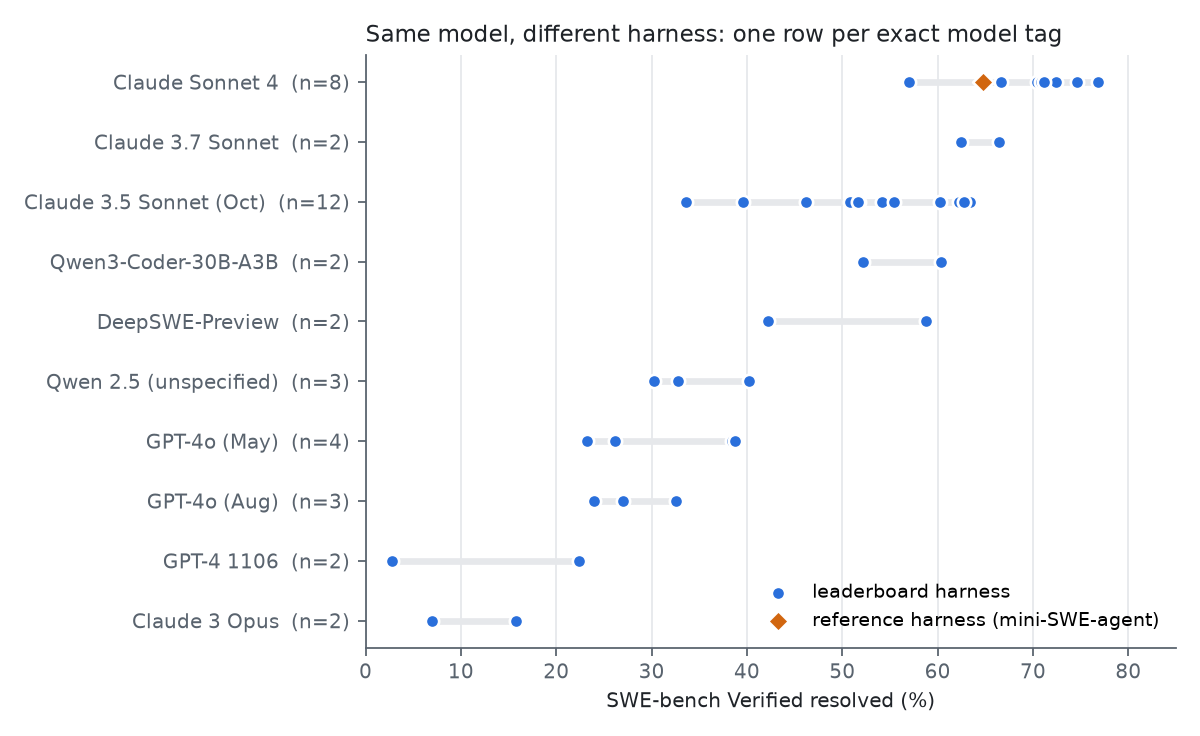
\includegraphics[width=0.92\linewidth]{fig1.png}
\caption{Every leaderboard submission on each exact model tag with at least two submissions (blue dots). Only Claude Sonnet 4 also has a complete reference-harness run (orange diamond).}
\label{fig:h1}
\end{figure}

Of 111 within-model pairs, 68 (61.3\%) are separable after Holm correction, and 85 have raw $p<0.05$ (Figure~\ref{fig:h1}, Table~\ref{tab:h1}). The pre-registered expectation was at least 50\%; H1 is supported. The median absolute difference is 8.2 points; the largest non-separable difference is 6.6 points.

\emph{Sensitivity (exploratory).} Removing the flagged rows (date-impossible tags, RAG baselines and the mixed ``Qwen 2.5'' tag) leaves 93 pairs in 7 models, of which 52 (55.9\%) are separable.

\begin{table}[t]
\centering
\caption{Same model, different harness. SWE-bench Verified resolved, \%. $\dagger$ marks a row or value affected by a data-quality flag (Section~\ref{sec:data}).}
\label{tab:h1}
\begin{tabular}{lrrrrr}
\toprule
model (exact tag) & submissions & best & median & worst & spread \\
\midrule
Claude Sonnet 4 (20250514) & 8 & 76.8 & 71.0 & 57.0 & 19.8 \\
Claude 3.7 Sonnet (20250219) & 2 & 66.4 & 64.4 & 62.4 & 4.0 \\
Claude 3.5 Sonnet (20241022) & 12 & 63.4 & 53.0 & 33.6$^\dagger$ & 29.8 \\
Qwen3-Coder-30B-A3B & 2 & 60.4 & 56.3 & 52.2 & 8.2 \\
DeepSWE-Preview & 2 & 58.8 & 50.5 & 42.2 & 16.6 \\
``Qwen 2.5''$^\dagger$ & 3 & 40.2 & 32.8 & 30.2 & 10.0 \\
GPT-4o (2024-05-13) & 4 & 38.8 & 32.3 & 23.2 & 15.6 \\
GPT-4o (2024-08-06) & 3 & 32.6 & 27.0 & 24.0$^\dagger$ & 8.6 \\
GPT-4 1106-preview & 2$^\dagger$ & 22.4 & 12.6 & 2.8 & 19.6 \\
Claude 3 Opus (20240229) & 2$^\dagger$ & 15.8 & 11.4 & 7.0 & 8.8 \\
\bottomrule
\end{tabular}
\end{table}

The widest rows are Claude 3.5 Sonnet, where eleven correctly tagged submissions span 23.8 points (the 33.6\% run carries the date-impossible tag), and Claude Sonnet 4, where eight submissions span 19.8 points. The DeepSWE and Qwen3-Coder-30B rows each compare one agent with and without test-time scaling; the GPT-4 1106 and Claude 3 Opus rows compare a RAG baseline with an agent.

\subsection{H3: the attempts confound}

Some submissions report the best of several attempts, which inflates their score relative to single-attempt runs. Restricted to pairs where both submissions used one attempt, 11 of 24 (45.8\%) are separable, in 4 models. The pre-registered expectation was at least one third; H3 is supported. The median difference is 4.4 points and the largest non-separable difference 4.6 points. With flagged rows also removed, 9 of 22 (40.9\%) are separable.

\subsection{How large is the harness relative to the model? (exploratory)}

Table~\ref{tab:var} decomposes the score variance over exact tags, using only groups with at least two submissions after each filter. Grouping by model \emph{family} inflates the harness share: pooling, say, all ``claude-4'' models counts size and snapshot differences as harness spread. This gives 0.62, and 0.67 on single-tag submissions, a figure previously reported from the same repository. With exact tags the within-model standard deviation is 0.39--0.45 of the between-model standard deviation. The ratio is specific to this sample (models with at least two harnesses, released over two years) and is a ratio of standard deviations; the corresponding variance ratio is about 0.15.

\begin{table}[t]
\centering
\caption{Between-model and within-model (harness) standard deviation of resolved \%, by grouping.}
\label{tab:var}
\begin{tabular}{lrrrrr}
\toprule
grouping & submissions & groups & between SD & within SD & ratio \\
\midrule
exact tag, all & 40 & 10 & 17.9 & 6.9 & \textbf{0.39} \\
exact tag, single attempt & 13 & 4 & 16.4 & 6.3 & 0.38 \\
exact tag, flagged rows removed & 31 & 7 & 13.8 & 6.2 & 0.45 \\
model family (regular expression) & 59 & 13 & 18.1 & 11.3 & 0.62 \\
\bottomrule
\end{tabular}
\end{table}

The mirror-image test is side B, where the harness is fixed and the model varies: 472 of 703 pairs (67.1\%) are separable, with a median difference of 11.8 points.

\subsection{H2: what a leaderboard harness adds on top of the reference harness}

Seven exact model tags have both a leaderboard submission and a complete reference-harness run (Table~\ref{tab:h2}). For five of them there is only one leaderboard submission, so ``best leaderboard harness'' means ``the only one''.

\begin{table}[t]
\centering
\small\setlength{\tabcolsep}{4pt}
\caption{Leaderboard harness versus the best reference-harness run of the same model tag. Resolved, \%. ``Flagged removed'' recomputes the gap over the 441 instances that no reference-harness run flagged for repository-history access. ``Later below'' counts reference-harness runs of later-released models that score below the leaderboard harness.}
\label{tab:h2}
\begin{tabular}{lrcrrlrr}
\toprule
model & leaderboard & $n$ & reference & gap & $p$ & flagged removed & later below \\
\midrule
Claude Sonnet 4 & 76.8 (2+ att.) & 8 & 64.8 & \textbf{+12.0} & $<10^{-4}$ & +11.3 & 30/31 \\
\quad best single attempt & 74.6 & & 64.8 & \textbf{+9.8} & $<10^{-4}$ & & \\
Kimi K2 Instruct & 53.4 & 1 & 43.8 & \textbf{+9.6} & $<10^{-4}$ & +9.5 & 2/30 \\
GPT-5 (20250807) & 71.8 & 1 & 65.0 & \textbf{+6.8} & $<10^{-4}$ & +7.7 & 13/23 \\
Claude Opus 4 & 73.2 & 1 & 67.6 & \textbf{+5.6} & 0.003 & +5.0 (4.99) & 25/31 \\
Claude Opus 4.5 (20251101) & 79.2 & 1 & 74.4 & +4.8 & 0.0005 & +5.4 & 13/13 \\
Gemini 3 Pro preview & 77.4 & 1 & 74.2 & +3.2 & 0.014 & +3.4 & 15/15 \\
Claude Opus 4.5 (undated) & 79.2 & 1 & 76.8 & +2.4 & 0.10 & +1.8 & 13/13 \\
\bottomrule
\end{tabular}
\end{table}

The pre-registered criterion was a separable gap of at least 5 points for at least half of the models. It is met for 4 of 7; H2 is supported, and six of the seven gaps are separable. The result is fragile. With the flagged instances removed the count is still 4 of 7, but the membership changes: Claude Opus 4 falls to 4.99 points and the dated Claude Opus 4.5 rises to 5.4. Two of the four qualifying gaps lie within a point of the threshold.

\begin{figure}[t]
\centering
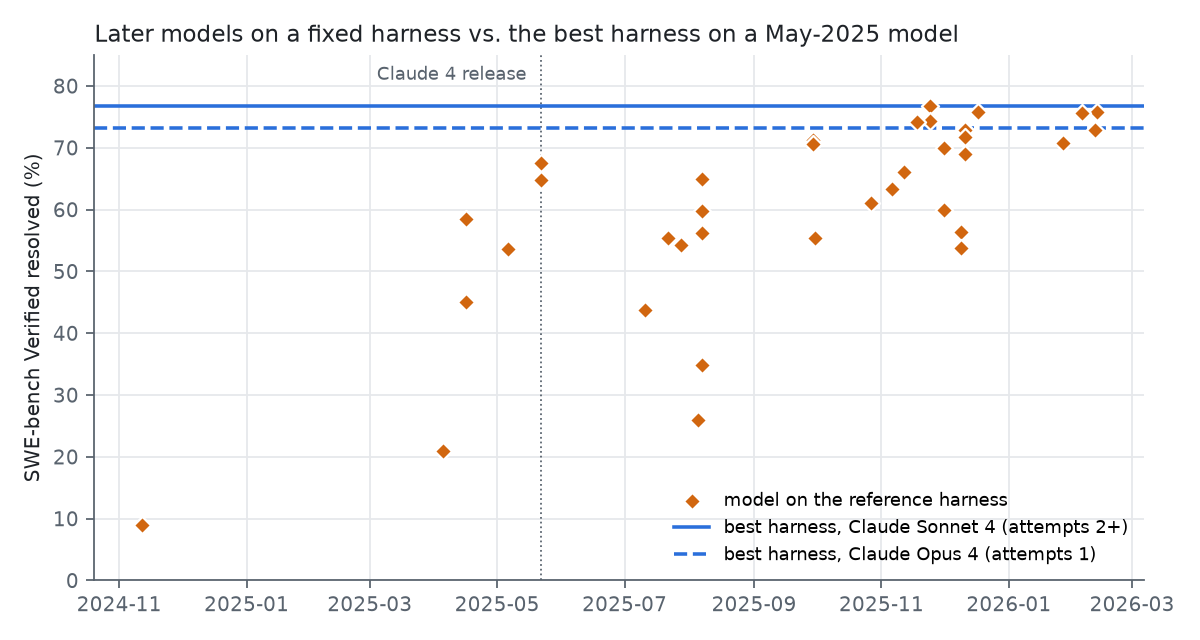
\includegraphics[width=0.92\linewidth]{fig2.png}
\caption{Every complete reference-harness run by model release date (orange), against the leaderboard harness on Claude Sonnet 4 and Claude Opus 4 (blue lines). Both models were released in May 2025.}
\label{fig:cal}
\end{figure}

\emph{Calendar reading (exploratory).} Claude Opus 4 has a single leaderboard harness, its developer's own single-attempt run at 73.2\%. Of 31 reference-harness runs of later-released models, 25 score below it (22 of 28 counted per model tag). On this record no reference-harness run reached 73.2\% until Gemini 3 Pro preview, released 18 November 2025, six months after Claude Opus 4 (Figure~\ref{fig:cal}). This is not a controlled comparison: the reference harness is deliberately minimal, its versions changed, and some later runs use high reasoning settings.

\subsection{H4: the reference-harness board itself}

On the reference-harness board only 4 of 37 adjacent ranks are separable after Holm correction (3 of 37 with flagged instances removed). No direction was pre-registered. Neighbouring ranks are rarely distinguishable even with the harness family held fixed.

\section{Discussion}

\paragraph{For open-weight models the harness gap on the record is widest.} The open-weight Kimi K2 scores 43.8\% on the reference harness and 53.4\% on a SWE-agent-based leaderboard harness ($+9.6$ points, $p<10^{-4}$). OpenHands on the July \texttt{kimi-k2-0711-preview} tag reaches 65.4\%; our pre-registered rule does not merge different tag strings, but these are very likely the same weights, and measured exploratorily the gap is $+21.6$ points ($p\approx5\times10^{-24}$). Devstral Small, small enough for a single consumer GPU, scores 46.8\% under OpenHands (May 2025 snapshot), 38.0\% under SWE-agent (July 2025 snapshot) and 56.4\% on the reference harness (December 2025 snapshot); these are different snapshots, so the comparison is not paired. Closed frontier models show gaps of 2--7 points, with Claude Sonnet 4 the exception.

\paragraph{The harness does not replace the model.} The between-model standard deviation is 2.2--2.6 times the within-model one, so a 20-point deficit is unlikely to close through harness work alone. On the minimal harness the best open-weight models are already close to the best closed model (MiniMax 2.5 at 75.8\% and GLM-5 at 72.8\%, against 76.8\%).

\paragraph{Harness claims should be tested.} About two in five same-model harness differences on the public record are not distinguishable from noise, including differences up to 6.6 points. Below 3 points only 1 of 21 within-model pairs is separable (0 of 20 with flagged rows removed). Following \citet{card2020power}, we recommend that agent papers report, next to ``$+X$ points'', the exact paired $p$-value and the smallest gap their comparison could have detected. Our tool \texttt{paircheck.py} computes both from two result files; for example, the largest H2 gap (76.8\% versus 64.8\%, with 68 against 8 discordant instances) could have detected a gap of 4.0 points.

\section{Limitations}

Model tags are self-reported and not checked against trajectories; two are date-impossible, and the same weights sometimes appear under different strings (Claude Opus 4.5, Kimi K2), so some real pairs go unused. The comparisons are not causal: harnesses arrive at different times with different budgets, and the reference harness changed version. H2 uses each model's best reference run, which is conservative for the gap. Seventeen of 55 bash-only runs are unusable; each is listed in the supplementary material. The study covers one benchmark with 500 instances, on which gaps below about 3 points are rarely resolvable. The maintainers' per-instance record ends in early 2026 (reference-harness logs to February 2026); per-sample logs from a third-party scaffold exist for newer models up to June 2026 and were not used, and we found no public per-instance results for later model families (checked November 2026).

\section{Reproducibility}

All inputs are public, and the analysis runs on a laptop in a few minutes after a one-off download of about 280\,MB of report files. The supplementary material contains the analysis scripts (H1 and H3 with parity check and flags; H2 and H4 with contamination sensitivity; the exploratory decomposition; figures), the per-run inclusion table, the original pre-registration with its hash and the deviation log, and \texttt{paircheck.py}.

\subsubsection*{Acknowledgments}
The SWE-bench maintainers publish per-instance results; none of these tests is possible without that.

\bibliography{main}
\bibliographystyle{tmlr}

\end{document}
